\documentclass[oneside]{book}
\usepackage{fullpage}
\usepackage{graphicx}
\usepackage{hyperref}
\usepackage{polyglossia}
\usepackage{xcolor}
\setdefaultlanguage[variant=american]{english}
\setotherlanguage[numerals=eastern]{farsi}
\setmainfont[Mapping=tex-text]{Linux Libertine O}
\newfontfamily\englishfont[Mapping=tex-text]{Linux Libertine O}
\newfontfamily\farsifont[Script=arab,Scale=1.25]{Scheherazade}

\usepackage{linguex}
\def\eg{e.g.,~}
\def\ie{i.e.,~}
\def\menu#1{\textsc{#1}}
\def\menu#1#2{\textsc{#1 | #2}}
\def\gloss{\textsf{Gloss}}
\def\sect#1{§\ref{#1}}

\def\p#1{\textfarsi{#1}}

\def\fig#1{Figure~\ref{#1}}

\definecolor{light-gray}{gray}{0.95}

\def\tip#1\par{\medskip\noindent\fcolorbox{black}{light-gray}{\parbox{\textwidth}{#1}}\par\medskip}


\title{\gloss\ User's Guide}
\author{Adam Baker}
\begin{document}
\maketitle
\tableofcontents

\chapter{Introduction}
\gloss\ is software for interlinearizing text and creating a lexicon. \gloss\ bears a strong resemblance to SIL's Language Explorer, to which it is indebted on several levels, but also has important differences. The most important of these are:

\begin{itemize}
\item \gloss\ is \emph{very fast} --- the program itself is very fast, but it also helps you to be very fast by automating 
\item \gloss\ allows for efficient revisions to the baseline text.
\item \gloss\ makes it easy to associate audio files with interlinear text, which is helpful for making revisions.
\item In addition to the graphical interface, all of the underlying data are accessible to the user, through SQL, XQuery, XSLT, and related technologies.
\item \gloss\ is agnostic as to whether the data are entered in orthography or transcription. Switching between these is simply a matter of looking at the data with a different view.
\item \gloss\ is created with Qt, a cross-platform development toolkit, so that \gloss\ can be run on *nix or Mac systems as well.
\end{itemize}

\gloss\ is the result of me freaking out about not having an acceptable tool for doing text interlinearization, and deciding to build one that will do the job. It's also the result of me interlinearizing texts for eight hours a day with my informant, and freaking out when a single thought required more than a single mouse click. So, the twin obsessions of \gloss\ are, i) getting the data structures right, and ii) creating a tool that works \emph{just} as it ought.

There are a lot of undocumented features in \gloss. Eventually this manual will become more thorough. If you're interested in something you see, feel free to send me an email. I have a pretty good response time for questions, bug reports, feature requests, etc.

\tip In this manual, random tips for doing things better are included in these shaded boxes.

\chapter{Getting started}
Launch \gloss. Begin a new project with \menu{File}{New Project}. You are prompted to choose a filename. Enter something like myproject.zip.

\section{Writing Systems}
You are first prompted to configure the writing systems of the project. Although you can edit these later, it is a good idea to get some in right away. You want to add a row to this table for every writing system in your project. And example is shown in \fig{fig:ws} For instance, if I were analyzing a text transcribed in Persian orthography, I would want to use three writing systems:

\begin{figure}
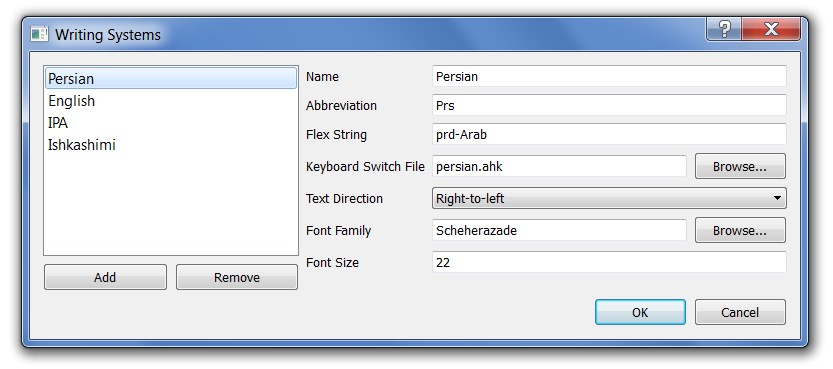
\includegraphics[width=\textwidth]{languages.png}
\caption{The writing system configuration dialog.}\label{fig:ws}
\end{figure}

\begin{itemize}
\item ``Persian Orthography''
\item ``Persian IPA Transcription''
\item ``English Orthography''
\end{itemize}
In this example, English orthography is included because that is the language with which I will be analyzing the data, \eg in glosses. For each writing system you need to fill in the cells of the table:

\begin{description}
\item[Name] Some name that a human can read
\item[Abbreviation] An abbreviation, which will be used to refer to the writing system when space is tight.
\item[Flex String] \emph{Important:} This should consist only of letters and hyphens (\ie no spaces or weird characters). Beyond that, there is no restriction on what the string is, other than that it is different from all of the others.
\item[Keyboard Switch File] You can leave this for now, but refer to  \sect{sect:switching-input-languages} for how to use this feature to switch your keyboard input automatically.
\item[Text Direction] Select the direction of the writing system.
\item[Font Family] The name of the font you want to use for the writing system.
\item[Font Size] The size of the font (in points) you want to use for the writing system.
\end{description}
Click OK to accept your writing system defaults. You'll be doing something with these on the next screen.

\section{Project Options}
This dialog requires you to add some high-level project options. Again, these can be set later, but it will be best to get them right the first time around. The demo configuration is shown in \fig{fig:po}.

\begin{figure}
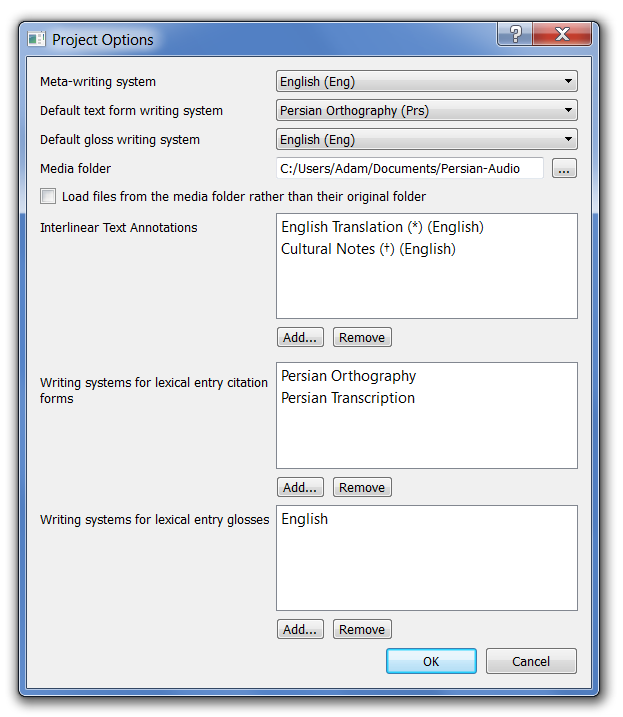
\includegraphics[width=\textwidth]{project-options.png}
\caption{The project options dialog.}\label{fig:po}
\end{figure}

\begin{description}
\item[Meta-writing system] This is the primary analysis language (probably the language in which you do your academic work).
\item[Default text form writing system] Depending on your texts, this might be the target language orthography or transcription.
\item[Default gloss writing system] This should be one of your analysis languages (\eg English for this example).
\item[Media folder] If all of your audio files are in a single folder, you can specify that folder here. It's not necessary to do so unless you check the next box...
\item[Load files from...] You can overload the paths to media files in your FlexText files, and load them from the Media Folder path instead.\footnote{This feature becomes relevant when you send your project to someone else, and all of a sudden all of the media files are in a different folder.}
\item[Interlinear Text Annotations] You can add annotations at every word, if you like. Specify a name for the annotation (which must be different from the names of the other annotations), a little symbol, and the writing system for the annotation.
\item[Writing ... citation forms] Add all of the writing systems for which your lexicon will have citation forms. Typically, these would be orthographic, and IPA transcription.
\item[Writing ... glosses] Add all of the writing systems for which your lexicon will have glosses (translations). This will be your analysis languages.
\end{description}
Click OK to move on and configure the views.

\section{View configuration}\label{sect:views}
Work from left to right in this dialog. For purposes of getting started, we'll have one view with two tabs; you can do more complex layouts later. The dialog is shown in \fig{fig:view}.

\begin{figure}
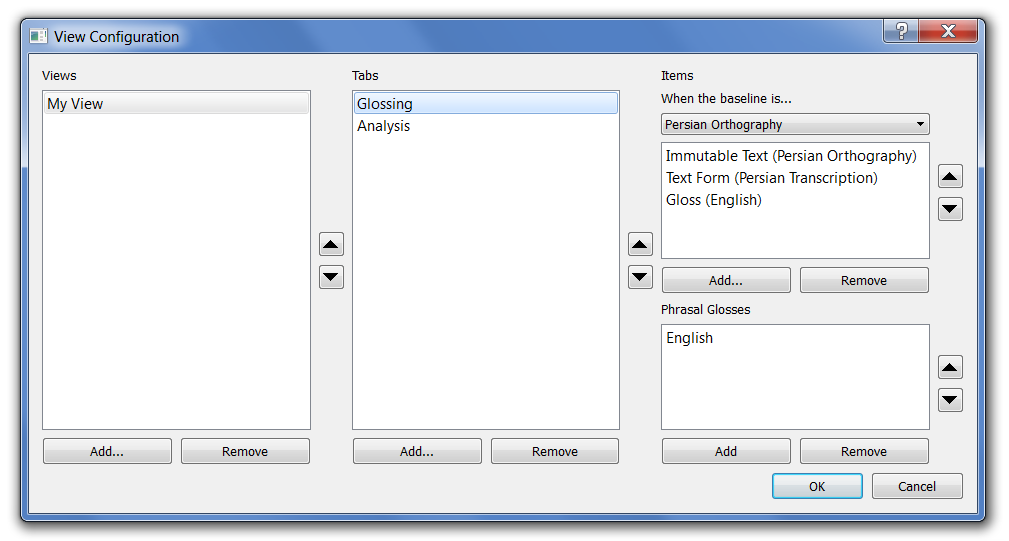
\includegraphics[width=\textwidth]{view-configuration.png}
\caption{The view configuration dialog.}\label{fig:view}
\end{figure}

Add a view with the ``Add...'' button, and give it a name (``My View'' in the example). It appears in the Views box. Click it.

Add a tab with the ``Add...'' button under the Tabs box, and give it a name (``Glossing''). Add another tab and call it ``Analysis.'' (For both of these, leave the default setting ``Interlinear'' unchanged.)

Under the Items box, click ``Add...'' to add a new line of interlinear text. This will require some thought. We will have a basic interface here, but more complexity is possible; see \sect{sect:types-of-interlinear-lines} for more detail.  For each item that we create, select ``Persian Orthography'' under ``For baseline text.'' Create one with Item Type ``Immutable Text'' and Writing System ``Persian Orthography.'' Create one with Item Type ``Text'' and Writing System ``Persian Transcription.'' Create one with Item Type ``Gloss'' and Writing System ``English.''

Next, under the Phrasal Glosses box, add one with ``English.'' The end result of these operations is illustrated in \fig{fig:view}.

Now select the ``Analysis" tab. Under Items, add an item. (Again, for each item that we create, select ``Persian Orthography'' under ``For baseline text.'') Create one with type ``Immutable Text'' and writing system ``Persian Orthography.'' Create one with type ``Immutable Gloss'' and writing system ``English.'' Create one with type ``Analysis'' and writing system ``Persian Transcription.''

Then, as before, under the Phrasal Glosses box, add one with ``English.''

Click OK. You are done with this part.

\section{Adding texts}
Although there are a number of ways to import texts into \gloss, we will follow the simplest: importing a plain text file.

I have a file un-prs.txt, a plain text file encoded in UTF-8. The text is the first article of the United Nations Declaration of Human Rights, translated into Persian. The text is broken up onto four lines:

\medskip
\begin{farsi}
\noindent
تمام افراد بشر آزاد زاده میشوند \\
و از لحاظ حیثیت و کرامت و حقوق با هم برابراند.\\
همگی دارای عقل و وجدان هستند \\
و باید با یکدیگر با روحیه ای برادرانه رفتار کنند.
\end{farsi}

\medskip
Select \menu{Texts}{Import plain text...}. \gloss\ prompts you to select a file. It next asks you for the baseline writing system of the text. For this example, the writing system is ``Persian Orthography.'' After a moment while \gloss\ digests the text, the interlinear text appears on the screen.

\subsection{Adding texts from Elan files}
One of the cooler features of \gloss\ is that it allows you to play sounds that go along with your text. If you have an Elan (.eaf) file, you can put that directly into \gloss. Do \menu{Texts}{Import EAF...} and select your .eaf file. You'll need to tell Gloss which tier you want to import.\footnote{This is shown at the left side of the Elan screen. In the Elan file, it is the value of the attribute ANNOTATION\_DOCUMENT/TIER/@TIER\_ID.} You'll also need to tell it the writing system of the text you're importing. Once this is done, you can open the text, double-click on a line number, and the sound for that line of text will be played.

\tip If, for some reason, you have an ELAN file with intervals that correspond to lines of text that you have imported some other way, then you can use \menu{Texts}{Merge EAF...} or \menu{Texts}{Bulk merge EAF...}. This will insert references to the audio files in your existing text.

\section{The interlinear interface}
The interface for editing interlinear texts looks like an interlinear text. \gloss\ has interpreted every line of text in un-prs.txt as an interlinear line. Here we see the results of our work in the Views Configuration dialog. We are currently in the ``Glossing'' tab; you can look at the ``Analysis'' tab, but there won't be much to see there yet. Note how the three lines of text are: a line of Persian orthographic text that you can't edit; an editable line of Persian transcription; and an editable English gloss line. This is what we set up in the last section; you can refer to \menu{Project}{Configure views...} to refresh your memory.

\tip The \gloss\ layout is intentionally clutter-free. If you forget what an entry is, just hover your mouse over the field, and a tool tip will pop up reminding you of the writing system.

The first word on line 2 is \p{و} [wæ] `and'. In the line immediately under the word, transcribe the word: wæ. Then hit the Tab key on your keyboard to go to the next word. Instantly, all of the instances of this word are transcribed. Enter the gloss: and. Again, as soon as you are finished, the gloss is filled in other places as well.

\tip When you fill in a gloss or a transcription, you're actually editing the database. That's what makes \gloss\ so fast. When you run into the situation where one entry needs more than one gloss or transcription, see Section~\ref{sect:homophones}.

The last word on line 3 is \p{هستند} [hæstænd] `they are.' Add this transcription and gloss. (This is the only instance of this word in the text, so nothing else updates.)

Now go to the Analysis tab. For the few words we have glossed, we can see the Persian orthography and the English gloss.\footnote{Again, look at \menu{Project}{Configure views...} to see how what we did in that dialog created what we see here.} For most of the words, there is nothing.

For one of the instances of  \p{و}, create a monomorphemic morphological analysis by clicking ``Monomorphemic.'' A form pops up; \gloss\ has made guesses about what the appropriate glosses and citation forms are, but you can edit these. You can also enter in grammatical information tags---anything you want, separated by spaces. When  you click OK, the morphological example is displayed.

For a more interesting morphological analysis, click ``Polymorphemic'' under \p{هستند}. \gloss\ presents the word in IPA transcription, asking you to indicate the morphological structure with various symbols.\footnote{It knows to do it in IPA, because in the \menu{Project}{Configure views...} dialog, we told it to use the Persian Transcription writing system.} To indicate that hæstænd is the stem hæst followed by the morpheme ænd, write: hæst -ænd.\footnote{This interface is borrowed directly from Language Explorer.} When you click OK, you see a list of the morphemes.\footnote{If you got the morpheme type wrong, you can change it in the drop-down box.} To create lexical entries, click ``Create new...'' next to each morpheme. The same analysis appears as before. In this case, Gloss can't guess what the orthography will be; it's guess for the gloss is probably wrong as well. We can assign a gloss ``COP'' for copula, and a citation form \p{هست} (you can type nonsense if you're unfamiliar with Persian, of course). Click OK, and then do the suffix. It's a 3P suffix, with the citation form \p{ند}. Click OK for that dialog. Click OK once more. Now the morphological analysis appears in the interlinear interface.

\chapter{Intermediate skills}

\section{Dealing with homophones/homonyms, alternate transcriptions, and alternate glosses}\label{sect:homophones}
Homophones and homonyms are relatively frequent in natural data. This section describes how to deal with them.

The Persian example text does not have any homophones that I'm aware of, but let's imagine that \p{و} could alternately be a word meaning `potato.' In that case, we need to decide for each instance of \p{و} whether it should be interpreted as one word or the other.

Right-click on the baseline text of one of the instances of \p{و}; a large context menu appears. We want the ``Interpretation'' submenu. Interpretations are important in \gloss: they permit the same text form to be interpreted multiple ways. We want to add a new interpretation, so do \menu{Interpretation}{New interpretation...}. Immediately, the transcription and gloss disappear; also, all of the other instances of \p{و} change color.

The blank fields are those of the new interpretation. We can transcribe [wæ] and gloss `potato.' \gloss\ has not changed any of the other transcriptions, but the change in color alerts us that there are \emph{multiple interpretations available} for the text form. Right-click on another instance of  \p{و} and select the ``Interpretation'' submenu. The various interpretations are listed, and you can select the `potato' interpretation if you wish. (If you do, the color changes to white, since you have made a decision about the item.)

\tip You can also hit the F1 key to cycle between all of the interpretations of a word. This saves a lot of mouse-work.

Alternate transcriptions or glosses work the same way. Persian \p{و} is sometimes pronounced [o]. If I want to change one of the instance of \p{و} to have that transcription (say, working from an audio recording), I right-click on the item and select \menu{Persian Transcription}{New text form...}. I can enter an alternate text form, and again from the same context menu I can select whichever variant I want. You can add variant glosses the very same way.

\tip When the cursor is in one of the line edits for a text form or gloss, you can press the keyboard's `Insert' key as a shortcut to add a new text form or gloss.

\tip To cycle between the transcriptions in this example, hit F2. To cycle between glosses you would hit F3. The generalization is: to change the interpretation F1, and then every line down is another function key.

\tip When there are multiple options for a a text form or gloss, the left edge of the box is colored blue. This can alert you to default values that you need to check.

For glosses, there is an option to ``Copy from baseline text...'' This is helpful in the case that you're working in a language with a lot of loan words from one of the gloss languages. It just saves you having to retype the word.

\section{Adding annotations}
You can add annotations to any word of a text. The system for adding or removing annotations is discussed in \sect{sect:views}. Once the annotations are added, they appear as light gray symbols occurring before the words. To add or edit an annotation, double click on the symbol. You can edit the annotation, and then click OK to save your changes. If a word has an annotation, the symbol for that annotation is shown in black instead of gray.

If you'd like to review all of the annotations associated with a text, you can use the annotation dock. Select \menu{Search}{Annotation dock...}. Select the annotation tier you want from the drop-down menu. Double click on an annotation to jump to that place in the text.

\section{Editing the baseline text}
One of \gloss's main strengths is that it allows you to edit the baseline text, without losing your work. This is necessary because all texts are bound to have transcriptional or typographic errors.

For instance, in the sample text, line 4 has two words \p{روحیه} and \p{ای}, where it should really have a single word: \p{روحیه‌ای}. (This sort of typo is quite common in Persian texts.) There are several ways to fix this:

\begin{itemize}
\item Right-click on the ``4'' line label and click ``Edit baseline text.'' This will give you a pop-up window, which you can edit however you wish. If you choose this option, though, any work you have done in choosing between alternate interpretations or glosses will be lost.
\item Right-click on \p{روحیه} and click ``Merge with next.'' This gives you a pop-up to edit. (In this case, one would want to edit the result to make the glyphs display properly.)
\item Right-click on \p{ای} and click ``Merge with previous.'' This is the converse of the previous.
\item Right-click on one of the words and click ``Edit baseline text,'' and then right-click on the other and click ``Remove.''
\end{itemize}

\chapter{Digging deeper}

\section{Basic concepts}
The difference between \emph{text forms} and \emph{glosses} is important in \gloss. A text form is an item of language data: it can be in the native orthography, or in IPA transcription. A gloss is an item of analysis: a gloss of the word in an analysis language. In the example below,\footnote{From the linguex documentation.} the English line has text forms, and the German line has glosses.

\exg. This is a first gloss\\
Dies ist eine erste Glosse\\

The same distinction would hold if the data were in IPA transcription: the first line has text forms, and the second line glosses.

\exg. ðɪs ɪz ə fɹst ɡlɑs\\
Dies ist eine erste Glosse\\

\section{Types of interlinear lines}\label{sect:types-of-interlinear-lines}
There are five types of lines of interlinear text.

\begin{itemize}
\item A \emph{Text} line creates an edit box for a text form. If you want a line of interlinear text that you can edit, use this type of line.
\item A \emph{Gloss} line creates an edit box for a gloss. If you want to be able to edit the gloss of a field, use this type of line.
\item \emph{Immutable Text.} This displays a text form, without giving the option to edit it. This can be helpful if you want to refer, \eg to an orthographic form, without the distraction of being able to edit it.
\item \emph{Immutable Gloss}. This displays a gloss, without giving the option to edit it. (This is parallel to an Immutable Text line.)
\item \emph{Analysis}. This displays a morphological analysis.
\end{itemize}

\section{Switching input languages automatically}\label{sect:switching-input-languages}
One of the biggest hassles in text interlinearization is having to switch the language of your keyboard: from the analysis language, to the native orthography, to IPA transcription. Wouldn't it be nice if \gloss\ did that for you?

This is a tricky subject because switching the input language has to do with your computer's operating system (Windows, Apple, etc.), so it's not straightforward. It's going to be different for different systems. What \gloss\ will do is try to run as a command whatever you have in the ``Keyboard Switch File'' entry of \menu{Project}{Writing systems...}. So for instance, in Windows I have a program that changes the keyboard input to Persian, so my ``Keyboard Switch File'' entry for Persian Orthography is the location of that executable:\\ \verb+C:\Users\Adam\Documents\QtWork\Gloss\persian.exe+

In a *nix or Apple system, I imagine that this would be done with a shell command. I give directions for Windows in the next section.

\subsection{Switching input languages in Windows}
This is obscure, but not terribly difficult. You will need to be able to use the command prompt to be able to do this. There is a freely-available scripting program called AutoHotKey.\footnote{\url{http://www.autohotkey.com/}}  You can make lots of different kinds of scripts with this program, but we're interested in changing the keyboard language.

I am going to demonstrate how to create an executable to change your keyboard to Icelandic, since that's a keyboard that a lot of linguists (presumably, not Icelandic linguists) use to hold their IPA keyboard.

\begin{itemize}
\item Download AutoHotKey and install it. Make a note of the installation location. Mine is \\ \verb+C:\Program Files (x86)\AutoHotkey+
\item Navigate to that location, and then to the Compiler folder. For me, that's\\ \verb+C:\Program Files (x86)\AutoHotkey\Compiler+
\item Create a simple text file called ``icelandic.ahk''. Put this text in that file:\\ \verb+PostMessage, 0x50, 0, 0x040F,, A+
\item Open a command window in that same folder.
\item Type this into the command window and hit enter:\\
\verb+Ahk2exe.exe /in icelandic.ahk+
\item Now there's a new executable that will change your keyboard to Icelandic:\\
\verb+C:\Program Files (x86)\AutoHotkey\Compiler\icelandic.exe+
\item Put that whole last line into the ``Keyboard Switch File''  in \menu{Project}{Writing systems...}.
\end{itemize}

How do you do this for other languages? You consult this web site: \url{http://msdn.microsoft.com/en-us/goglobal/bb896001} This has a long list of languages, with a hexidecimal code in the leftmost column (like 0x040F). If you scroll down to Icelandic, the code to the left of it is 0x040F. If I wanted to create an executable to switch the import language to Persian, I would replace 0x040F with 0x0429 in the code above: \verb+PostMessage, 0x50, 0, 0x0429,, A+

No kidding, this is really how it works!

\section{Searching}
To search your texts, do \menu{Search}{Search dock...}. This calls up the search dock, at the right of the screen. (You may be prompted to build the index first; click `Yes.') From the search dock you can search for anything in your texts.

For instance, if I want to find all instances of the word \p{وجدان} in my texts, I select ``Persian Orthography'' from the writing systems, type the word, and hit Enter. Another dock appears on the left, showing that this work occurs just once. If I double-click that, a one-line editor pops up showing me the line of text.

If I right-click on the search result, there are further options. ``Edit Line'' is the default behavior. ``Edit Line With Context'' will show me Line 3, with a line before and a line after. ``Open Text'' will open the entire text. ``Play Sound'' will play the sound associated with the file, if there is one.

From the dock ``Substring search'' is available if you want to search for part of a word or gloss. For instance, I select ``Persian Transcription'' and type ``æs'' and---with the ``Substring search'' box checked---it calls up the transcribed word ``hæstænd.''

You're also able to search by database id, in case that is helpful. This will be useful for users thinking carefully about the database.

\subsection{The Search Index}
By default, \gloss\ searches an index rather than the texts themselves. This makes things go faster. If you prefer the slower method, you can select \menu{Search}{Search files instead of index}. Judge for yourself; if the number of texts is small, the difference may not be very important.

\gloss\ will try to guess when the index needs to be updated, \eg after texts are added to the project. But if you've just completed a big chunk of glossing, you may want to select \menu{Search}{Rebuild index}. This takes a while, so it's only worth doing it every once in a while.

\subsection{Approved and Unapproved Lines}
In interlinear text mode, the baseline word is typically colored green or yellow. The idea here is that you can ``approve'' a line by double-clicking on the colored box, whereupon it turns white. You can use this to keep track of your progress in a text. It means nothing more than what you want it to.

To find lines that have unapproved (\ie colored) words, click \menu{Search}{Search for unapproved lines}. To find lines that have approved (\ie white) words, click \menu{Search}{Search for approved lines}.

\section{Syntactic Analysis}
\gloss\ allows you to create syntactic annotations from your texts, once you've done a morphological analysis. The syntactic analysis groups the morphemes together into larger constituents.

\gloss\ is agnostic about your syntactic theory, by the way. It doesn't require that the elements of a constituent be contiguous, or about any of the syntactic categories.

\subsection{Getting Started}
To do a syntactic analysis, you need to create a syntactic analysis tab. Go to the View Configuration window with \menu{Project}{Configure views...}. With a certain view selected, click ``Add'' to add a tab. Under ``Type of tab,'' select ``Syntactic Annotation'' (instead of ``Interlinearlization''). Give the tab a name like ``Syntax.''

With that tab selected, click ``Add'' under ``Items.'' These next settings are not intuitive. For the baseline text, select the writing system for the baseline; in this case, we would select ``Persian Orthography'' since that is the writing system of our texts. Under ``Item Type'' select ``Analysis,'' and then ``Persian Transcription'' for the next box. This is because our morphological analysis uses transcribed Persian (IPA).

Click ``Add'' again, and add a line with Item Type ``Gloss'' and writing system ``English.'' Click OK. Now click OK again to leave the View Configuration window.

When you open the text again, you will have the ``Syntax'' tab. No analysis is shown because you have not created one. At the bottom of the tab, click ``Add...'' Add a name for the analysis, and change the writing system to ``Persian Transcription.'' This is because our morphological analysis is in Persian transcription. Leave ``Closed Vocabulary'' unchecked for now. Click OK, and the screen fills with text.

\tip The syntactic analysis depends on your morphological analysis, so you need to do your morphophonemic analysis first. Or, if you modify your morphophonemic analysis, click the ``Refresh Text'' button in the syntactic analysis window.

\tip \gloss\ doesn't know what a word is because I don't know what a word is. The syntactic analysis is performed directly on morphemes. If you wish, you can make the first constituents correspond to word-level morphological categories. As a phonologist, I can only anticipate that this will be gratifying to some syntacticians and vexing to others.

\subsection{Annotating}
Any of the morphemes can be selected using the mousey-dragging-rectangle method. Select a constituent's worth of morphemes, and press A (for `Add'). Type a label for the constituent, press OK, and the constituent appears.

To delete a constituent, select it and hit `X'. \gloss\ will only try to delete an element if you select a \emph{single} element. (You can't delete your morphemes, of course.)

To add things to a constituent, you can select them and then drag/drop them onto another constituent.

\subsection{Synchronizing your morphophonemic analysis}
Your syntactic analysis is a grouping of morphemes, so if you morphological analysis changes, you need to update the text. This is done with the ``Refresh Text'' button. Some day this may become automatic, but for now it is manual. \gloss\ will retain as much of the analysis as it can, given the changed morphemes.

\subsection{Annotating with a fixed vocabulary}
Perhaps you want a little more structure in your annotations: a fixed vocabulary of syntactic elements. To do it that way, check the ``Closed Vocabulary'' box when you're setting up an analysis. Then you'll need to set up the closed vocabulary with \menu{Project}{Syntactic elements...}. (This dialog works just like the \menu{Project}{Writing systems...} dialog.)

\begin{description}
\item[Abbreviation] This is the label that will be shown in the tree display.
\item[Name] So far, this is not used.
\item[Keyboard shortcut] Very helpful. You can create a keyboard shortcut to add your elements.
\item[Automatic parent] Perhaps your theory of syntax requires every N to have an NP parent. Then you can create an N element and an NP element, and set NP as the ``automatic parent'' of N. Then when you create an N element (perhaps with the shortcut key `N'), it will automatically add the NP. 
\end{description}

While annotating with a fixed vocabulary, use the keyboard's Delete button to delete constituents. The `X' key is reserved in case you want to make it a shortcut.

\tip For automatic parenting, \gloss\ isn't smart enough to know if you create a circular (\ie infinite) parenting like N $\to$ NP $\to$ N $\to ...$. So don't mess that up. 

\chapter{Advanced use}

\gloss's internal workings are open to plain view. This section has the information you need to make things happen that \gloss\ can't already do. All of this comes with the disclaimer: make sure you have a back-up!

\section{The ``Under the hood'' menu}
The ``Under the hood'' menu provides convenient access to the database menu. A few highlights... 

Use \menu{Under the hood...}{View/Edit SQL Tables...} to see what's in the database, and to modify it if you wish. Use  \menu{Under the hood...}{Perform a SQL query...} to perform any query on the database (select; update; delete; drop; whatever!).

\menu{Under the hood...}{Raw XQuery...} is intended to enable you to search the XML files with XQuery, but currently it is not working well. I doubt there's any way to searching the files that would be less difficult.

\section{Types of files}
\gloss\ stores your project in a Zip archive. You can give the project file any extension you want; it remains a Zip archive. If you trust yourself, you can modify the contents of any of these files. Of course, it is a good idea to make a back-up in case you make a mistake.

When \gloss\ opens a file, it opens the Zip archive and puts the contents in a temporary directory. On Windows, for instance, when I open the file ``Wakhi.zip,'' \gloss\ creates this temporary directory:  \url{C:/Users/Adam/AppData/Local/Temp/Gloss-WLD.zip}. If you like, you can modify the files directly. If you save the project, Gloss will create the archive from those files.

Texts are stored in FlexText files (.flextext), a file format adopted directly from SIL's Language Explorer. FlexText files are XML files, entirely suitable for archival purposes. Typically these files only contain numerical references to the database. You can tell \gloss\ to write the data there, but for that you probably want to do \menu{File}{Export texts...}

\gloss\ stores other data (text forms, glosses, morphological analyses, lexical information, etc.) in a SQLite3 database.\footnote{\url{http://www.sqlite.org/}} This is a lightweight and open source SQL database system. The database file is called sqlite3-database.db.

\subsection{Gloss's FlexText files}
SIL's FlexText file format is an excellent way to represent interlinear texts, so there was no need to reinvent the wheel for this project. For various applications, however, it was necessary to add elements and attributes beyond SIL's format. To keep things tidy, my own elements come with the namespace \url{http://www.adambaker.org/gloss.php} (or, as I abbreviate it, ``abg''). If you strip everything from that namespace out of the file, you will be a pure SIL-style FlexText file. Bear in mind, however, that if you strip out the elements with that namespace, \gloss\ won't be able to read the file.

\subsection{File Encoding}
UTF-8. \gloss\ works with text in UTF-8 encoding, from beginning to end. All SQL data are encoded in UTF-8; all XML files are encoded in UTF-8. All data that you import need to be encoded in UTF-8.

\end{document}